\section{Tema 1 - Estadística descriptiva}

\begin{problem}[2] Demostrar que \[ \sum_{i=1}^n \left(x_i-\avg{x}\right)^2 = \min_{a\in \real} \sum_{i=1}^n(x_i-a)^2 \]

\solution

Definimos una función \[ g(a) = \sum_{i=1}^n(x_i-a)^2 \], buscamos su derivada \[ g'(a) = -2 \sum_{i=1}^n(x_i-a) \] e igualamos a cero:

\begin{gather*}
-2 \sum_{i=1}^n(x_i-a) = 0 \\
\sum_{i=1}^n x_i - \sum_{i=1}^n a = 0 \\
n \avg{x} = n a \\
\avg{x} = a 
\end{gather*}

Esto quiere decir que la media muestral es el valor que minimiza la distancia con cada uno de los datos de la muestra.
\end{problem}

\begin{problem}[5]Determina si es verdadero o falso:

\ppart Si añadimos 7 a todos los datos de un conjunto, el primer cuartil aumenta en 7 unidades y el rango intercuartílico no cambia.

\ppart Si todos los datos de un conjunto se multiplican por -2, la desviación típica se dobla.
\solution 

\spart Añadir siete a todos los datos es una traslación, así que la distribución de los datos no cambia.

\spart Teniendo en cuenta que si multiplicamos todos los datos del conjunto por $-2$ la media también se multiplica por $-2$, y sustituyendo en la fórmula de la varianza:

\[ \sigma' = \sqrt{\frac{1}{n} \sum_{i=1}n (-2x_i)^2 - (-2\avg{x})^2} = \sqrt{\frac{1}{n} \sum_{i=1}4\left(n x_i^2 - \avg{x}^2\right)} = \sqrt{4\sigma^2} = 2\sigma \]

Por lo tanto, la desviación típica sí se dobla.

\spart Usando los cálculos del apartado anterior vemos que la varianza se multiplica por cuatro.

\spart Efectivamente: cambiar el signo haría una reflexión de los datos sobre el eje Y y la asimetría estaría orientada hacia el lado contrario. 

\end{problem}

\section{Tema 2 - Muestreo aleatorio}

\begin{problem}[1] Se desea estimar el momento de orden 4, $\alpha_3 = \esp{X^3}$ en una v.a. $X$ con distirbución exponencial de parámetro 2, es decir, la función de distribución de $X$ es $F(t) = \prob{X ≤ t} = 1 - e^{-2t}$ para $t≥0$. Definir un estimador natural para $\alpha_3$ y calcular su error cuadrático medio.

\solution

Usando el criterio de \textit{plugin}, podríamos definir el estimador \[ \hat{\alpha}_3 = \int_\real x^3\,d\fd_n(x) \]. 

Calculamos ahora el error cuadrático medio:

\begin{gather*}
ECM(\hat{\alpha}_3) = \esp{\hat{\alpha}_3 - \alpha_3}^2 = \esp{(\hat{\alpha}_3 - \esp{\hat{\alpha}_3} + \esp{\hat{\alpha}_3} - \alpha_3) ^2} = \\
= \esp{(\hat{\alpha}_3 - \esp{\hat{\alpha_3}})^2 +  (\esp{\hat{\alpha_3}}- \alpha_3)^2 + 2(\hat{\alpha}_3 - \esp{\hat{\alpha_3}}) (\esp{\hat{\alpha_3}}- \alpha_3)} = \\
= \underbrace{\esp{(\hat{\alpha_3} - \esp{\hat{\alpha_3}})^2}}_{(a)}+ \underbrace{\left(\esp{\hat{\alpha_3}} - \alpha_3\right)^2}_{(b)} + \underbrace{2 \cdot \esp{ (\esp{\hat{\alpha_3}}- \alpha_3)^2 + 2(\hat{\alpha}_3 - \esp{\hat{\alpha_3}})}}_{(c)} 
\end{gather*}

Aquí ya hay cosas raras. (c) es cero por alguna razón, luego hay que calcular la varianza y el sesgo.

\[ \text{sesgo}(\hat{\alpha}_3) = \esp{\hat{\alpha}_3} - \alpha_3 = \alpha_3 - \alpha_3 = 0 \]

\[ \var{\hat{\alpha}_3} = \var{\frac{1}{n}\sum X_i^3 } = \frac{1}{n^2}\var{\sum X_i^3} = \frac{1}{n^2}\sum \var{X_i^3} = \frac{\var{X^3}}{n} \]

y, teniendo en cuenta el enunciado,

\[ \var{X^3} = \esp{X^6} - \esp{X^3}^2 = \frac{6!}{2^6} - \left(\frac{3!}{2^3}\right)^2 = \frac{171}{16} \]

y por lo tanto

\[ \text{ECM}(\hat{\alpha}_3) = \frac{171}{16n} = O(\frac{1}{n)} \convs 0 \]

donde lo que más nos importa es la convergencia a cero, que indica que cuanto más muestras tenemos mejor será el estimador.

\end{problem}

\begin{problem}[2] Supongamos que la muestra tiene tamaño $n=50$ y que la distribución de las $X_i$ es una $N(4,1)$. 

\ppart Obtener, utilizando la desigualdad de Chebichev, una cota superior para la probabilidad $\prob{\abs{\avg{X} - 4} > 0.3}$.

\ppart Calcula exactamente $\prob{\abs{\avg{X} - 4} > 0.3}$ utilizando la distribución de $X_i$. 

\solution
\spart

Como la media es cuatro, la desigualdad de Checbichev nos da una cota de 

\[ \frac{\var{\avg{x}}}{0.3^2} = \frac{\var{X}}{n \cdot 0.3^2} \simeq 0.22 \]

\spart

Normalizamos

\[ Z = \frac{\avg{X} - 4}{\frac{1}{\sqrt{50}}} ~ N(0,1) \]

y calculamos.

\[ \prob{\abs{\avg{X} - 4} > 0.3} = \prob{\abs{Z} > \frac{0.3}{\frac{1}{\sqrt{50}}}} = 2 \cdot \prob{Z > 2.12} = 0.038 \]

\end{problem}

\begin{problem}[4] Denotemos por 

\[ C_n = \int_\real \left(\fd_n(t) - F(t)\right)^2 \, dF(t) \]

la llamada discrepancia de Cramer-Von Mises entre $\fd_n$ y $F$. ¿Converge a cero casi seguro esta discrepancia?

Calcular la distribución asintótica de la sucesión $D_n = \sqrt{n}\left(\fd_n(t) - F(t)\right)$ para un valor fijo $t\in\real$.

\solution

\[ C_n = \int_\real \left(\fd_n(t) - F(t)\right)^2 \, dF(t) = \int_\real \left(\fd_n(t) - F(t)\right)^2 f(t) \, dt \]

Como por el teorema de Glivenko-Cantelli (\ref{thmGlivenko}) tenemos que 

\[ \fd_n(t) - F(t) ≤ \sup_t \abs{\fd_n(t) - F(t)} = \md{\fd_n - F}_\infty \]

entonces 

\[ \int_\real \left(\fd_n(t) - F(t)\right)^2 f(t) \, dt ≤  \md{\fd_n - F}_\infty^2 \int_\real f(t) \,dt = \md{\fd_n - F}_\infty^2 \]

Igualmente por Glivenko-Cantelli, 

\[ \md{\fd_n - F}_\infty^2 \convcs 0  \qed \]

\spart

Para calcular la distirbución asintótica de \[ D_n = \sqrt{n}\left(\fd_n(t) - F(t)\right) \] usamos el Teorema Central del Límite (\ref{thmCentral}). Necesitamos algo que se asemeje a una media muestral, y de hecho

\[ \fd_n(t) = \frac{1}{n} \sum_{i=1}^n \ind_{(-\infty, t]} (X_i) = \frac{1}{n} \sum_{i=1}^n Y_i = \avg{Y} \]

Por otra parte, $Y = \ind_{(-\infty, t]}(X)$ y por lo tanto \[ \esp{Y} = \esp{\ind_{(-\infty, t]}(X)} = \prob{X ≤ t} = F(t) \]

Ya podemos aplicar el TCL, pero nos falta saber cuál es la desviación típica de $Y$. Como es una distribución de Bernoulli 

\[ \mathbb{V}(Y) = p(1-p) = F(t)(1-F(t)) \]

y por lo tanto 

\[ D_n \convdist N\left(0, \sqrt{F(t)(1-F(t))}\right) \]
\end{problem}

\begin{problem}[5] Sea $X$ una v.a. cuya función de densidad depende de un parámetro desconocido $\theta \in \real$, concretamente \[ f(x;\theta) = \frac{1}{\pi}\frac{1}{1+(x-\theta)^2} \] para $x\in \real$. Comprobar que $\theta$ coincide con la mediana y la moda de $X$ pero que la media $\esp{X}$ no está definida.

Diseñar un experimento de simulación en R, tomando algún valor concreto de $\theta$, orientado a comprobar cómo se comportan la mediana muestral y la media muestral como estimadores de $\theta$: mientras la mediana muestral se acerca al verdadero valor de $\theta$ al aumentar $N$, la media muestral oscila fuertemente y no se acerca a $\theta$ aunque se aumente el tamaño muestral $n$.

\solution Viendo la función, vemos que es simétrica con respecto al eje $x= \theta$. Por lo tanto, el punto que deja a izquierda y derecha la misma probablidad, la mediana, es precisamente $\theta$. 

De la misma forma, la moda es el valor máximo de la distribución, que se ve claramente que ocurre cuando $x=\theta$.
\end{problem}

\begin{problem}[7] Sea $X$ una v.a con distribución absolutamente continua. Sea $F$ la correspondiente función de distribución y $f = F'$ continua en todo punto la función de densidad. para $r\in \{1,\dotsc,n\}$, denotemos por $X_{(r)}$ el $r$-simo estadístico ordenado de una muestra de tamaño $n$ extraída de $X$. Calcular la función de distirbución y la de densidad de la v.a. $X_{(r)}$.

\solution

Por definición

\[ F_{X_{(r)}} (x) = \prob{X_{(r)} ≤ x }\]

que es la probabilidad que al menos $r$ elementos de la muestra sean menores o iguales que $x$. Luego la probabilidad es igual a

\begin{gather*}
\sum_{j=r}^n \prob{\text{exactamente j observaciones de la muestra son ≤ x}} =  \\
= \sum_{j=r}^n \prob{B(n, F(x)) = j} = \sum_{j=r}^n \comb{n}{j}F(x)^j \left(1 - F(x)\right)^{n-j}
\end{gather*}

Ahora sólo falta calcular la densidad de $X_{(r)}$, y la obtenemos derivando

\begin{gather*}
 f_{X_{(r)}} (x) = \\
 = \sum_{j=r}^n \left(\comb{n}{j}j(F(x)^{j-1}(1-F(x))^{n-j}f(x) - (F(x))^j(n-j)(1-F(x))^{n-j-1} f(x)\right) = \\
 = \sum_{j=r}^n \comb{n}{j} j(F(x)^{j-1}(1-F(x))^{n-j}f(x)  - \sum_{j=r}^n\comb{n}{j} (F(x))^j(n-j)(1-F(x))^{n-j-1} f(x) = \\
 = \comb{n}{r} r(F(x))^{r-1} (1-F(x))^{n-1}f(x) + \sum_{j=r+1}^n \comb{n}{j}j(F(x))^{j-1} f(x) (1-F(x))^{n-j} \\
 \quad \quad - \sum_{j=r}^n\comb{n}{j}(n-j)(F(x))^j (1-F(x))^{n-j-1}f(x) = \\
 n\comb{n-1}{r-1}(F(x))^{r-1} (1-F(x))^{n-r} f(x)    +   \sum_{l=r}^{n-1}n\comb{n-1}{l}(F(x))^l (1-F(x))^{n-l-1} f(x) \\
 \quad\quad -  \sum_{j=r}^{n-1}n\comb{n-1}{j}(F(x))^j (1-F(x))^{n-j-1} f(x)
\end{gather*} 

Los dos últimos términos se cancelan y nos queda que 

\[ f_{X_{(r)}} (x) = n\comb{n-1}{r-1}(F(x))^{r-1} (1-F(x))^{n-r} f(x) \]

Consideremos los dos casos particulares del mínimo y máximo de la muestra. Con el mínimo, $r=1$ y entonces

\[ F_{X_{(1)}} (x)= \prob{X_{(1)} ≤ x} = \sum_{j=1}^n\comb{n}{j}(F(x))^j(1-F(x))^{n-j} = 1 - (1-F(x))^n \]

En el caso del máximo:

\[ F_{X_{(n)}} (x) = \prob{X_{(n)} ≤ x } = (F(x))^n \]

\end{problem}

\begin{problem}[8] Sea $\hat{f}_n$ un estimador kernel de la densidad basado en un núcleo $K$ que es una función de densidad con media finita. Comprobar que, en general, $\hat{f}_n(t)$ es un estimador sesgado de $f(t)$ en el sentido de que \textbf{no} se tiene $\esp{\hat{f}_n(t)} = f(t)$ para todo $t$ y para toda densidad $f$.

\solution

\begin{gather*}
\esp{\hat{f}_n(t)} = \esp{\frac{1}{nh}\sum_{i=1}^n K \left(\frac{t-X_i}{h}\right)} = \\
= \frac{1}{nh}\sum_{i=1}^n \esp{K\left(\frac{t-X_i}{h}\right)} = \frac{1}{h} \esp{K\left(\frac{t-X}{h}\right)} = \\
= \frac{1}{h} \int_\real K \left(\frac{t-x}{h}\right) f(x) \,dx = 
\end{gather*}

Haciendo un cambio de variable $x = t-hz$, $dx = -h\,dz$, los límites se invierten,

\[ = \frac{1}{h} \int_{-\infty}^\infty K \left(\frac{t-x}{h}\right) f(x) \,d(x)  = \frac{-1}{h} \int_\infty^{-\infty} K(z) f(t-hz) h \,dz  = \int_{-\infty}^\infty Kz f(t-hz)\,dz \]

Ahora buscamos calcular el sesgo:

\[ \text{sesgo}\,(\hat{f}_n(t)) = \esp{\hat{f}_n(t)} - f(t) = \]

Usando que $K$ es función de densidad y que $\int K = 1$, nos queda

\begin{gather*}
 = \int_{-\infty}^\infty K(z) f(t-hz)\,dz - \int_{-\infty}^\infty K(z) f(t)\, dz = \\
 = \int_{-\infty}^\infty K(z) \left[f(t-hz)-f(t)\right]\,dz =\\
 = hf'(t)\int_{-\infty}^\infty zK(z)\,dz + \frac{1}{2} h^2 f''(t) \int_{-\infty}^\infty z^2K(z)\,dz + \frac{1}{6}h^3 f'''(t) \int_{-\infty}^\infty z^3K(z)\,dz + \dotsb  
\end{gather*}

al hacer el desarrollo de Taylor. Como $K$ es una función simétrica, las integrales con índice impar (con $z=1, 3,\dotsc$) se anulan. Sin embargo, el segundo término no lo hace. Por lo tanto, el sesgo de un estimador kernel \textbf{no es nunca cero}. 

El sesgo del estimador kernel depende de $h$ (el parámetro de suavizado o \textit{bandwith}) en potencias pares. Por eso, se toma de manera tal que $h\convs 0$ y entonces $\text{sesgo}\,\hat{f}_n(t) \convs 0$ pero manteniendo un equilibrio para que la varianza también sea pequeña y no tengamos picos en el histograma (ver sección \ref{secEst}).

\end{problem}
\section{Tema 3 - Estimación puntual paramétrica}

\begin{problem}[3] Se disponeb de un gran lote de piezas producidas en una cadena de montaje. Denotemos por $p$ la proporción de piezas defectuosas en ese lote. Supongamos que se seleccionan al azar sucesivamente (con reemplazamiento) piezas del lote hasta que se encuentra una defectuosa. Sea $X$ la variable aleatoria que indica el número de la extracción en la que aparece la primera pieza defectuosa.

\ppart Calcular $\prob{X=k}$ para $k=1,2,\dotsc$ Obtener el estimador de $p$ por el método de los momentos, a partir de una muestra $X_1,\dotsc , X_n$.

\ppart Obtener el estimador de $p$ por el método de máxima verosimilitud. Calcular su distribución asintótica.
\solution
\spart
La probabilidad sigue una distribución geométrica de parámetro $p$:

\[ \prob{X=k} = (1-p)^{k-1}p \]

\spart Calculamos la función de verosimilitud:

\[ L(p;x_1,\dotsc,x_n) = \prod_{i=1}^n f(x_i;p) = \prod_{i=1}^n (1-p)^{x_i -1}p = (1-p)^{\sum_{i=1}^n x_i -n} p^n \]

Tomamos logaritmos

\[ \log L(p) = \log(1-p) \left(\sum_{i=1}^n x_i -n\right) + n\log p \]

y derivando

\[ \deriv{}{p} \log L(p) = \frac{-1}{1-p} \left(\sum_{i=1}^n x_i -n\right)  + \frac{n}{p} \] 

y derivas tú lo que queda, majo.
\end{problem}

\begin{problem}[5]
Distribución de Rayleigh, cuya función de densidad es:
\[f(x;\theta) = \frac{x}{\theta^2} e^{\frac{-x^2}{2\theta^2}} \mathbb{I}_{[0,\infty)} (x), \theta > 0\]

\begin{itemize}
\item[a]Calcular el estimador de máxima verosimilitud (e.m.v.)
\item[b]Calcular la consistencia.
\item[c] ¿Es asintóticamente normal?
\end{itemize}

\solution

\paragraph{a)}

\[L_n(\theta;x_1,...,x_n) = \frac{x_1 \cdot ... \cdot x_n}{\theta^2} e^{\frac{-1}{2\theta^2} \sum_{i=1}^n x_i^2}\]
\[log L_n(\theta) = \sum log x_i - 2nlog\theta -\frac{1}{2\theta^2}\sum x_i^2\]
\[\dpa log L_n(\theta) = \frac{1}{\theta} \left(-2n+\frac{1}{\theta^2}\sum x_i^2\right) = 0\]
\[\implies \hat{\theta}^2 = \frac{\sum x_i^2}{2n} \implies \hat{\theta} emv(\theta) = (\frac{\sum x_i^2}{2n}^2\]

Estimador razonable porque $E(x^2) = V(x) + E(x) = 2\theta^2 \dimplies \theta^2 = \frac{1}{2} E(x^2)$

\paragraph{b)}
\textbf{Consistencia:} $\hat{\theta}^2 = \frac{1}{2} \gor{Y}, Y_i = X_i^2$

Por la ley fuerte de los grandes números (\ref{thmGrandes}) sabemos que: $\gor{Y} \convs[cs] E_{\theta}(Y) = E_{\theta}(X^2) = 2\theta^2$

Vamos a aplicar el teorema de Snouschky?.

Sea $g(x) = \sqrt{\frac{1}{2}x}$ definida sobre $[0,\infty)$.

Teorema de Snoopy $\implies g\left(\gor{Y}\right) = \sqrt{\frac{1}{2} \frac{\sum x_i^2}{n}} \convs[c.s.] g(E_{\theta}) = \sqrt{\frac{1}{2}\theta^2} = \theta \implies $ El e.m.v. de $\theta$, $\hat{\theta}$ es consistente c.s.


\paragraph{c)}

Queremos aplicar el método delta:

\[\sqrt{n}(\hat{\theta} - \theta) = \sqrt{n}\left(g\left(\gor{Y}\right) - g\left(E(Y)\right)\right) \convs[d]N(0,\abs{g'(E(Y))}\sqrt{V(Y)}\]

\[E_{\theta}(Y) = E_{\theta} (X^2) = 2\theta^2\]
\[V_{\theta}(Y) = E(X^4) - E^2(X^2) = 8\theta^4-4\theta^4 = 4\theta^4\]

Entonces tenemos que $g'(E(Y)) = \displaystyle \frac{1}{2\sqrt{2E(Y)}} = \frac{1}{4\theta}$.

Con esta información completamos:  

\[\sqrt{n}(\hat{\theta} - \theta) \convs[d] N\left(0,\sqrt{\frac{1}{2\theta}}\right)\]

\end{problem}

\begin{problem}[11]
\footnote{Este ejercicio es del parcial del año pasado}

ashkjdf
\solution

$X\leadsto Unif[0,\theta]$
Con \[ f(x) = \displaystyle\left\{\begin{array}{cc}
\frac{1}{\theta} & 0\leq x \leq \theta\\
0 & x \notin [0,\theta]
\end{array}\right.\]

Vamos a calcular la función de distribución:

\[F_{\theta} (x) = \mathbb{P}_{\theta}\{X\leq x\} = \int_{-infty}^x f_{\theta}(t)dt = \int_0^x \frac{1}{\theta} dt = \frac{x}{\theta} \ si 0\leq x \leq \theta\]

\[F_{\theta} = \left\{\begin{array}{cc}
\frac{x}{\theta} & 0\leq x \leq \theta\\
0 & x \notin [0,\theta]
\end{array}\right.\]

Nos piden dibujar las funciones... GUILLEEEE xD

Vamos a calcular \[L_n(\theta;x_i) = \prod_{i=1}^n f_{\theta} (x_i) = \left\{\begin{array}{cc}
\left(\frac{1}{\theta}\right)^n & \forall x_i \in [0,\theta]\\
0 & \exists x_i\notin [0,\theta]
\end{array}\right.\]

Calculamos la $logL_n$ que nos piden dibujarla:

\[logL_n(\theta) = \left\{\begin{array}{cc}
-nlog(\theta) & si \ max(\{x_i\})\leq \theta\\
0 & si \ no
\end{array}\right.\]
Dibujoo!

\[\hat{\theta_n} = e.m.v.(\theta) = max\left(L_n(\theta)\right)\]

También vale tomando el logaritmo:

\[\hat{\theta}_n = e.m.v. (\theta) = arg\ mas logL_n(\theta) = max\{x_i\}\]
porque \[ logLn(\theta) = \displaystyle\left\{\begin{array}{cc}
-nlog(\theta) & max\{x_i\} \leq \theta\\
-\infty & si \ no
\end{array}\right.\]
\end{problem}

\begin{problem}[5]
Distribución de Rayleigh, cuya función de densidad es:
\[f(x;\theta) = \frac{x}{\theta^2} e^{\frac{-x^2}{2\theta^2}} \mathbb{I}_{[0,\infty)} (x), \theta > 0\]

\ppart Calcular el estimador de máxima verosimilitud (e.m.v.)

\ppart Calcular la consistencia.

\ppart ¿Es asintóticamente normal?

\solution

\spart

\[L_n(\theta;x_1,...,x_n) = \frac{x_1 \cdot ... \cdot x_n}{\theta^2} e^{\frac{-1}{2\theta^2} \sum_{i=1}^n x_i^2}\]
\[log L_n(\theta) = \sum log x_i - 2nlog\theta -\frac{1}{2\theta^2}\sum x_i^2\]
\[\dpa log L_n(\theta) = \frac{1}{\theta} \left(-2n+\frac{1}{\theta^2}\sum x_i^2\right) = 0\]
\[\implies \hat{\theta}^2 = \frac{\sum x_i^2}{2n} \implies \hat{\theta} emv(\theta) = (\frac{\sum x_i^2}{2n}^2\]

Estimador razonable porque $E(x^2) = V(x) + E(x) = 2\theta^2 \dimplies \theta^2 = \frac{1}{2} E(x^2)$

Buscamos ahora el estimador $\tilde\theta$ por el \textbf{método de los momentos}

\[ \esp[\theta]{X}= \theta\sqrt{\frac{\pi}{2}} = \avg{X} \] 

y entonces el estimador es \[\tilde{\theta} = \avg{X}\frac{2}{\pi} \]

\spart

\textbf{Consistencia:} $\hat{\theta}^2 = \frac{1}{2} \gor{Y}, Y_i = X_i^2$

Por la ley fuerte de los grandes números (\ref{thmGrandes}) sabemos que: $\gor{Y} \convs[cs] E_{\theta}(Y) = E_{\theta}(X^2) = 2\theta^2$

Vamos a aplicar el teorema de Slutsky.

Sea $g(x) = \sqrt{\frac{1}{2}x}$ definida sobre $[0,\infty)$.

Teorema de Slutsky (\ref{thmSlutsky}) $\implies g\left(\gor{Y}\right) = \sqrt{\frac{1}{2} \frac{\sum x_i^2}{n}} \convcs g(E_{\theta}) = \sqrt{\frac{1}{2}\theta^2} = \theta \implies $ El e.m.v. de $\theta$, $\hat{\theta}$ es consistente c.s.


\spart

Queremos aplicar el método delta:

\[\sqrt{n}(\hat{\theta} - \theta) = \sqrt{n}\left(g\left(\gor{Y}\right) - g\left(E(Y)\right)\right) \convs[d]N(0,\abs{g'(E(Y))}\sqrt{V(Y)}\]

\[E_{\theta}(Y) = E_{\theta} (X^2) = 2\theta^2\]
\[V_{\theta}(Y) = E(X^4) - E^2(X^2) = 8\theta^4-4\theta^4 = 4\theta^4\]

Entonces tenemos que $g'(E(Y)) = \displaystyle \frac{1}{2\sqrt{2E(Y)}} = \frac{1}{4\theta}$.

Con esta información completamos:  

\[\sqrt{n}(\hat{\theta} - \theta) \convs[d] N\left(0,\sqrt{\frac{1}{2\theta}}\right)\]

Buscamos ahora la convergencia asintótica del estimador por el método de los momentos:

\[ \sqrt{n}(\tilde\theta-\theta) = \sqrt{n}\left(\avg{X}\frac{2}{\pi}  - \esp{X}\frac{2}{\pi}\right) = \sqrt{\frac{2}{\pi}}\sqrt{n}(\avg{X}-\esp{X}) \]

que, por el TCL (\ref{thmCentral})

\[ \sqrt{\frac{2}{\pi}}\sqrt{n}(\avg{X}-\esp{X})  \convdist  \sqrt{\frac{2}{\pi}}N\left(0,\theta\sqrt{\frac{4-\pi}{2}}\right) = N\left(0,\theta\sqrt{\frac{4-\pi}{\pi}}\right) \]

y por lo tanto es efectivamente asintóticamente normal.

\end{problem}

\begin{problem}[11]
\footnote{Este ejercicio es del parcial del año pasado}

asdasdf
\solution

$X\leadsto Unif[0,\theta]$
Con $f(x) = \displaystyle\left\{\begin{array}{cc}
\frac{1}{\theta} & 0\leq x \leq \theta\\
0 & x \notin [0,\theta]
\end{array}\right.$

Vamos a calcular la función de distribución:

\[F_{\theta} (x) = P_{\theta}\{X\leq x\} = \int_{-infty}^x f_{\theta}(t)dt = \int_0^x \frac{1}{\theta} dt = \frac{x}{\theta} \ si 0\leq x \leq \theta\]

\[F_{\theta} = \left\{\begin{array}{cc}
\frac{x}{\theta} & 0\leq x \leq \theta\\
0 & x \notin [0,\theta]
\end{array}\right.\]

Nos piden dibujar las funciones... GUILLEEEE xD

Vamos a calcular \[L_n(\theta;x_i) = \prod_{i=1}^n f_{\theta} (x_i) = \left\{\begin{array}{cc}
\left(\frac{1}{\theta}\right)^n & \forall x_i \in [0,\theta]\\
0 & \exists x_i\notin [0,\theta]
\end{array}\right.\]

Calculamos la $logL_n$ que nos piden dibujarla:

\[logL_n(\theta) = \left\{\begin{array}{cc}
-nlog(\theta) & si \ max(\{x_i\})\leq \theta\\
0 & si \ no
\end{array}\right.\]
Dibujoo!

\[\hat{\theta_n} = e.m.v.(\theta) = max\left(L_n(\theta)\right)\]

También vale tomando el logaritmo:

\[\hat{\theta}_n = e.m.v. (\theta) = arg\ mas logL_n(\theta) = max\{x_i\}\]
porque \[ logLn(\theta) = \displaystyle\left\{\begin{array}{cc}
-nlog(\theta) & max\{x_i\} \leq \theta\\
-\infty & si \ no
\end{array}\right.\]
\end{problem}

\begin{problem}[2]
\[X\leadsto N(0,\sqrt{\theta}), \theta>0, Espacioparametrico = (0,\infty)\]
\solution
\paragraph{a)}
\[L_n(\theta;X_1,...,X_n) = \prod_{i=1}^n f(x_i;\theta) = \frac{1}{\sqrt{2\pi}^{\frac{n}{2}}\theta^{\frac{n}{2}}} e ^ {-\frac{1}{2\theta} \sum x_i^2}\]

\[logL_n(\theta) = \frac{n}{2}\cdot log(2\pi) - \frac{n}{2}log(\theta) - \frac{1}{2\theta} \sum x_i^2\]

\[\dpa{}{\theta} logL_n(\theta) = ... \implies T_n = e.m.v.(\theta) = \frac{1}{n}\sum x_i^2\]


b) $\esp[\theta]{T_n} = \esp[\theta]{\frac{1}{n}\sum x_i^2} = \esp[\theta]{X^2} = \theta$

Vamos a calcular la información de fisher para comprobar si el estimador es eficiente o no.

\[ log f(x;\theta) = \frac{-1}{2}log(2\pi)-\frac{1}{2}log(\theta) - \frac{1}{2\theta}X^2\]
Derivamos:
\[\dpa{}{\theta} log f(x;\theta) = -\frac{1}{2\theta} + \frac{1}{2\theta^2}X^2\]
Elegimos derivar otra vez o elevar al cuadrado (2 alternativas para calcularlo).

En este caso vamos a elevar al cuadrado:

\[\dpa{}{\theta}logf(X;\theta) = \frac{1}{4\theta} \left( 1+\frac{X^4}{\theta} - 2\frac{X^2}{\theta}\right)\]

Entonces la información de fisher será:

\[I(\theta) = \esp[\theta]{\frac{1}{4\theta} \left( 1+\frac{X^4}{\theta} - 2\frac{X^2}{\theta}\right)} = \frac{1}{4\theta} \left( 1+\frac{\esp[\theta]{X^4}}{\theta} - 2\frac{\esp[\theta]{X^2}}{\theta}\right)\]

Aplicamos por hipótesis: $\esp[\theta]{X^4} = 3\theta^2$

\[I(\theta) = \frac{1}{4\theta^4} \left(1+\frac{3\theta^3}{\theta^2} - 2 \frac{\theta}{\theta}\right) = \frac{1}{2\theta}\]

Vamos a calcular \[\var[\theta]{T_n} = \var[\theta]{\frac{1}{n}\sum x_i^2} = \frac{1}{n^2}\sum \var[\theta]{x_i^2} = \frac{n}{n^2} \var[\theta]{X^2} = \frac{1}{n}\left(\esp[\theta]{X^4} - \esp[\theta]{X^2}\right) = \frac{1}{n}(3\theta^2-\theta^2) = \frac{2\theta^2}{n} = \frac{1}{nI(\theta)} \implies EFICIENTEEE!\]

Los siguientes pasos para comprobar lo bueno que es el estimador son: \begin{itemize}
\item $T_n$ asintóticamente normal.
\item $T_n$ es consistente casi seguro.
\end{itemize}

\paragraph{c)} Vamos a estudiar la distribución asintótica:

\[\sqrt{n}(T_n-\theta) \convs[d] N(0,\sigma(\theta))\]

Llamando $Y_i = X_i^2 \implies \esp[\theta]{Y} = \esp[\theta]{X^2} = \theta$

Entonces: $\displaystyle \sqrt{n}(\hat{Y} - \esp[\theta]{Y}) \convs[TCL \ d] N(0,\sqrt{\var{Y}})$

Donde $\var{Y} = \var[\theta]{X^2} = 2\theta^2$
\end{problem}

\begin{problem}[8] Sea $X \sim N(µ,\sqrt{\theta})$. Estamos interesados en la estimación de $\theta$ basados en muestras $X_1,\dotsc,X_n$ de tamaño $n$. Calcular la cota de Fréchet-Cramer-Rao (\ref{thmCotaFCR}) para estimadores insesgados.

\solution

La cota FCR es \[ \frac{1}{n I(\theta)} \]

Podíamos calcular la información de Fisher como

\[ I(\theta) = \esp{\left(\dpa{}{\theta}\log f(X;\theta)\right)^2} = - \esp{\frac{∂^2}{∂\theta^2}\log f(X;\theta)} \]

Usaremos la segunda expresión. Calculamos primero el logaritmo:

\[ \log f(X;\theta) = \frac{-1}{2}\log 2\pi - \frac{1}{2}\log \theta - \frac{1}{2\theta}(x-µ)^2 \]

y derivamos dos veces

\begin{gather*}
 \dpa{}{\theta} \log f(X;\theta) = \log f(X;\theta) = -\frac{1}{2\theta} + \frac{1}{2\theta^2}(x-µ)^2 \\
 \frac{∂^2}{∂\theta^2} \log f(X;\theta) = \frac{1}{2\theta^2} - \frac{2}{2\theta^3} (x-µ)^2 = \frac{1}{\theta^2} \left(\frac{1}{2} - \frac{1}{\theta}(x-µ)^2\right) 
 \end{gather*}
 
 Calculamos ahora la esperanza:
 
 \[ \esp{\frac{1}{\theta^2} \left(\frac{1}{2} - \frac{1}{\theta}(x-µ)^2\right) } = -\frac{1}{\theta^2}\left(\frac{1}{2} - \frac{1}{\theta} \underbrace{\esp{X-µ}^2}_{\theta}\right) = \frac{1}{2\theta^2} \]
 
 y por lo tanto la cota FCR vale $\dfrac{2\theta^2}{n}$, el valor mínimo.

\end{problem}

\begin{problem}[9] Sea $X_1,\dotsc,X_n$ una muestra de una v.a. con función de densidad 

\[ f(x;\theta) = \theta x^{\theta - 1} \]

Sea  \[ T_n(X_1,\dotsc,X_n) = \frac{-1}{n}\sum_{i=1}^n\log X_i \]

\ppart Probar que \[\esp[\theta]{T_n} = \frac{1}{\theta};\; \var[\theta]{T_n} = \frac{1}{n\theta^2} \]
\ppart ¿Es eficiente $T_n$ como estimador de $\frac{1}{\theta}$?

\solution

\spart

\[ \esp[\theta]{T_n} = -\esp[\theta]{\log X} = - \int_0^1 \log x \theta x ^{\theta-1}\,dx = \frac{1}{\theta} \]

Calculamos ahora la varianza:

\begin{gather*}
\var[\theta]{T_n} = \frac{1}{n\theta^2} = \esp[\theta]{T_n^2} - \esp[\theta]{T_n}^2 = \frac{\var[\theta]{\log X}}{n} = \\
= \esp[\theta]{\log^2 X} - \esp[\theta]{\log X}^2 = \frac{1}{\theta^2}
\end{gather*}

\end{problem}

\section{Tema 4 - Intervalos de confianza}

\begin{problem}[1 y 2]
\textbf{a)}Representa un estimador de la función de densidad de la v.a. X = cantidad de contaminación por mercurio (en p.p.m.) en los peces capturados en los ríos norteamericanos Lumber y Wacamaw (ver fichero Datos-mercurio.txt). Comparar esta densidad estimada con la densidad normal de igual media y desviación típica (representada en la misma gráfica). En vista de las dos funciones dirías que la función de densidad de X es aproximadamente normal?

\textbf{b)} Obtener un intervalo de confianza de nivel 0.95 para la media de X.

\textbf{c)} Se puede considerar fiable este intervalo a pesar de la posible no-normalidad de X?

\textbf{d)} Qué tamaño muestral habrá que tomar para estimar la contaminación media con un error máximo de 0.06?
\solution
Solucionado por Amprao, descargable 
\href{http://www.uam.es/personal_pdi/ciencias/abaillo/MatEstI/T4DatosMercurio.pdf}{aqui}

\end{problem}

\begin{problem}[3]
\ppart Representa en un mismo gráficp las densidades de las distribuciones $\chi^2_k $ con k = 4,8,20,30.
\ppart $X \sim \gamma(5,10)$. Calcular $\mathbb{P}\{X\leq 3\}$
\ppart Sea $Y \sim \chi_{200}^2$. Calcular $\mathbb{P}\{Y\leq 3\}$

\solution
\spart
El código R utilizado para generar las gráficas es:
> x = seq(0,20,length.out=1000)

> d1=dchisq(x,df=4)

> d2=dchisq(x,df=8)

> d3=dchisq(x,df=10)

> d4=dchisq(x,df=20)

> plot(x,d1,type='l')

> lines(x,d2,type='l',col='blue')

> lines(x,d3,type='l',col='green')

> lines(x,d4,type='l',col='red')


\begin{center}
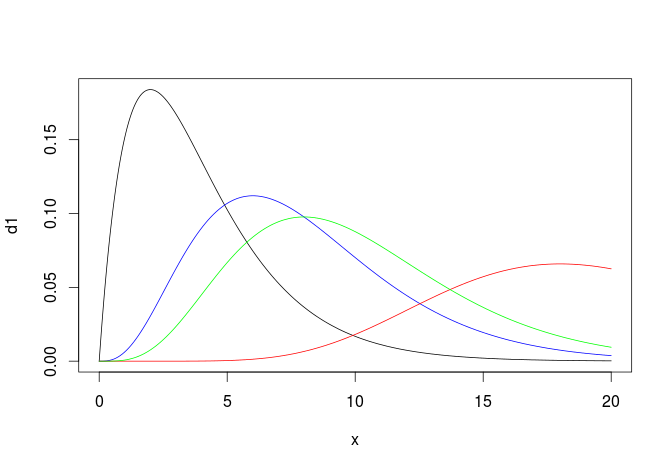
\includegraphics[width=1\textwidth]{Chicuadrado.png}
\label{Ejercicio 4}
\end{center}

\spart
Vamos a usar el resultado visto en clase:
Si $X\sim \gamma(a,p)$ entonces tenemos que 
\[cX \sim \gamma(c\cdot a, p)\]

En este caso, tomando $c=10$ tenemos:

\[\mathbb{P}\{10X\leq 30\} = \mathbb{P}\{\chi^2_{20 }\leq 30\}  \]

Tenemos varias opciontes. Una de ellas es ir a R y calcularlo con el comando \emph{pchisq(30,20)} = 0.93

Y la otra es irse a las tablas y vemos que $\mathbb{P}\{\chi^2_{20} \leq 30\} \simeq 0.93$

\spart Sea $Y \sim \chi_{200}^2$ 

Podemos hacerlo en R directamente y nos da $\mathbb{P}\{Y\leq 3\} = 10 ^{-141}$

A mano, aplicamos el T.C.L, que dice:
\[\sqrt{n}(\gor{X} - \mu) \convs[d] N(0,\sigma)  \]

Entonces tenemos: $\gor{X} \sim N\left(\esp{X},\displaystyle \sqrt{\frac{\var{X}}{n}}\right)$

Donde $\esp{X} = \esp{Z^2} = \var{Z} = 1$ y $\var{X} = \var{Z^2} = \var{\chi_1^2} = 2$

Con lo que:
\[\gor{X} \sim N\left(1,\frac{1}{10}\right)\]

Sustituyendo y estandarizando:

\[
\mathbb{P}\{\gor{X}\leq\frac{3}{20} \} \simeq \mathbb{P} \{Z\leq \frac{\frac{3}{200} - 1}{\frac{1}{10}} \} = \mathbb{P} \{Z\leq -9.85\} = 3 \cdot 10^{-23}
\]

Una diferencia bastante distinta a lo que decía R. Tras un debate entre Miguel y Amparo de 10 minutos no se ha llegado a ninguna conclusión.
\end{problem}

\begin{problem}[4]
\ppart Utilizando el fichero Datos-lipidos.txt, estima, mediante un intervalo de confianza de nivel
0.95, la proporción de pacientes que tienen una concentración de colesterol superior o igual a
220 mg/dl. ¿Qué tamaço muestral habrá que usar para tener una probabilidad aproximada de 0.95 de no cometer un error mayor que 0.01 en la estimación de esta proporción?

\ppart
\solution
Solucionado por Amprao, descargable 
\href{http://www.uam.es/personal_pdi/ciencias/abaillo/MatEstI/T4DatosLipidos.pdf}{aqui}
\end{problem}
\begin{problem}[5] Sea una v.a. con función de densidad $f(x;\theta) = \theta x^{-(\theta) + 1}\ind_{[1,\infty)} $

\ppart Obtener el e.m.v.

\ppart Obtener su distribución asintótica

\ppart Calcular la cantidad pivotal aproximada y, a partir de ella, un intervalo de confianza de nivel aproximada $1-\alpha$ para $\theta$
\solution
\spart \[\dpa{logL(\theta)}{\theta} = 0 \implies e.m.v.(\theta) = \frac{1}{\gor{Y}}\]
donde $Y = log X_i$

\spart Posibles caminos:

a) $\hat{\theta} \convs[d] $¿?

b) \[\sqrt{n}(\hat{\theta} - \theta) \convs[d] N\left(0,?\right)\]

La primera opción es algo difusa y la segunda es mucho más concreta y mejor.

Tenemos que examinar la expresión $\sqrt{n}(\hat{\theta} - \theta)$
Tenemos 2 posibilidades con las que calcular este tipo de cosas (T.C.L) y método delta (que es el que emplearemos a continuación)

\[\mu = \esp{X}; \sigma = \var{X}\]
\[\sqrt{n}\left(g(\gor{X}) - g(u)\right) \convs N(0,\abs{g'(u)} \sigma\]

Aplicando el método delta:

\[
\sqrt{n}(\hat{\theta} - \theta) = \sqrt{ n}\left(g(\gor{y})-g(\esp{Y})\right)\convs[d] N\left(0,\underbrace{\abs{g'\left(\frac{1}{\theta}\right)}}_{\theta^2} \sqrt{\var{Y}}\right) = N(0,\theta)
\]

Peeero... hay que tener cuidado con que $\theta = g(\esp{Y})$ porque sino no podemos aplicar el método delta.

\[
\var{Y} = \esp{Y^2} - \esp{^2 Y} = \underbrace{\int_1^2 (log\,x)^2 \theta x^{-(\theta + 1)}dx}_{\displaystyle\frac{2}{\theta}} - \frac{1}{\theta^2} = \theta{1}{\theta^2}
\]

\spart
La cantidad pivotal les un estadístico que depende de la muestra y del parámetro desconocido (del que estamos calculando el intervalo) y cuya distribución, al menos asintóticamente) es totalmente conocida.

En el apartado b) hemos encontrado la distribución asintótica para poder construir la cantidad pivotal.

Tipificamos el resultado anterior para evitar que la distribución depende del parámetro desconocido.

\[
\frac{1}{\theta} \sqrt{n}(\hat{\theta} - \theta)  = 
\sqrt{n} \left(\frac{\hat{\theta}}{\theta} - 1 \right) = \mathbb{Q}(\theta;X_1,...,X_N)
\]

Esta es nuestra cantidad pivotal, que depende de la muestra (por el $\hat{\theta}$) y depende del parámetro.

\[1-\alpha  = \mathbb{P} = \{q_1(\alpha) \leq \mathbb{Q}(\theta;X_1,...,X_N) \leq q_2 (\alpha)\}\]


El despejar se deja como ejercicio para el lector.

\end{problem}

\begin{problem}[6]
Sea $\sample$ una muestra de una v.a. uniforme en el interalo $[0,θ]$ con $0 < θ < 1$. Obtener una cantidad pivotal para $θ$ a partir del emv. Usando esta cantidad pivotal construye un intervalo de confianza para $θ$ de nivel prefijado $1-α$.

\solution

El e.m.v es \[ emv (θ) = \hat{θ} = \max X_i \] La cantidad pivotal para $θ = Q(θ; \sample)$

\[ F_{X_{(n)}} (x) = \prob{\hat{θ}_n ≤ x} = \prob{X_{(n)} ≤ x} = \prod_{i=1}^{n} \prob{X_i ≤ x} = \begin{cases}
0& x<0 \\
\left( \frac{x}{θ} \right)^n & 0≤x≤θ \\
1 & x > 1
\end{cases}\]

Tomo $Q(θ; \sample ) = \dfrac{X_{(n)}}{θ} = \dfrac{\hat{\theta}}{n}$, que es válido como cantidad pivotal porque \[ \prob{Q≤x} = \prob{\frac{X_{(n)}}{θ} ≤ x} = \begin{cases}
0 & x<0 \\
x^n & 0≤x≤θ \\
1 & x > 1
\end{cases} \]

Tenemos que elegir dos valores $q_1, q_2$ de tal forma que 

\[ 1- α = \prob{q_1(α) ≤ Q(θ;\sample) ≤ q_2(α)} \]

¿Cómo elegirlos? Queremos buscar que la longitud del intervalo de confianza $IC_{1-α}(θ) = \left(\dfrac{\hat{θ}_n}{q_2},\dfrac{\hat{θ}_n}{q_1}\right)$ sea mínima. Calculamos esa longitud:

\[ \text{len IC} = \hat{θ}_n\left(\frac{1}{q_1}-\frac{1}{q_2}\right)=\hat{θ}_n \left(\frac{q_2-q_1}{q_1q_2}\right) \]

Es decir, tenemos que buscar que $q_1-q_2$ sea más pequeño y además tienen que ser lo mayores posible. Por lo tanto, la elección óptima es 

\[ q_2 = 1,\;q_1=α^{1/n} \]

\end{problem}

\begin{problem}[7] Construye tres intervalos de confianza asintóticos diferentes para el parámetro $λ$ de una distribución de Poisson usando los tres métodos siguientes:

\ppart Utiliza el comportamiento asintótico de la media muestral, estima de forma consistente la varianza y aplica el teorema de Slutsky.

\ppart Igual que el anterior, pero sin estimar la varianza

\ppart Aplicando el método delta para \textit{estabilizar la varianza}, es decir, buscando una función $g$ tal que $\sqrt{n}(g(\avg{X}) - g(λ))\convdist N(0,1)$.

\solution

\spart El TCL (\ref{thmCentral}) nos dice que

\[ \sqrt{n}\frac{\avg{X} - λ}{\sqrt{λ}} \convdist N(0,1) \]

Entonces tenemos que 
\begin{equation}
 1-α = \prob{-z_{α/2}≤\sqrt{n}\frac{\avg{X} - λ}{\sqrt{λ}} ≤ z_{α/2}} \label{eqEj7}
 \end{equation}

Sustituyo $λ$ en el denominador por una estimación consistente $\hat{λ}\convs[P, c.s]λ$:

\[ \sqrt{n}\frac{\avg{X} - λ}{\sqrt{\hat{λ}}} \convdist N(0,1) \]

Como sabemos que $λ=\esp{X}$, tomamos la media muestral como el estimador: $\hat{λ} = \avg{X}$. La convergencia nos queda entonces como


\[ \sqrt{n}\frac{\avg{X} - λ}{\sqrt{\avg{X}}} \convdist N(0,1) \]

y por lo tanto tomamos $ \sqrt{n}\dfrac{\avg{X} - λ}{\sqrt{\avg{X}}}$ como nuestra cantidad pivotal. Despejamos ahora en (\ref{eqEj7}):

\[ \prob{\avg{X} - z_{α/2} \sqrt{\frac{\avg{X}}{n}} 
	≤ λ
	≤ \avg{X} + z_{α/2} \sqrt{\frac{\avg{X}}{n}}}
	\]
	
\spart Partimos de nuevo de (\ref{eqEj7}), pero no tenemos que estimar $λ$. Esta ecuación es equivalente a 

\[ \prob{n\frac{(\avg{X}-λ)^2}{λ} ≤ z_{α/2}^2} \]

De ahí sólo tenemos que despejar $λ$ para hallar nuestro intervalo de confianza.

\spart Tenemos que buscar que se satisfaga la ecuación \[ \sqrt{n}(g(\avg{X}) - g(λ))\convdist N(0,1) \]

Sin embargo, el método delta (\ref{defMetDelta}) nos dice algo distinto:

\[ \sqrt{n}(g(\avg{X}) - g(λ))\convdist N(0,\abs{g'(μ)}\sqrt{\var{X}}) \]

Entonces tenemos que 

\[ \abs{g'(λ)}\sqrt{λ} = 1 \implies g'(λ) = \frac{1}{\sqrt{λ}} \]

e integrando vemos que $g(λ) = 2\sqrt{λ} $.
\end{problem}

\begin{problem}[8]
\ppart Se desea evaluar aproximadamente, por el \textit{método de Montecarlo}, la integral 

\[ p = \int_0^1f(x)\,dx \] 

de una función continua $\appl{f}{[0,1]}{[0,1]}$. Para ello se generan 500 observaciones independientes $(X_i,Y_i)$ con $i=1,\dotsc,500$ con distribución uniforme en el cuadrado $[0,1]×[0,1]$ y se estima $p$ mediante

\[ \hat{p} = \sum_{i=1}^{500} \frac{Z_i}{500} \]

donde la v.a. $Z_i$ vale 1 si $Y_i≤f(X_i)$ y $0$ en caso contrario. ¿Qué distribución tienen las $Z_i$? Suponiendo que, en una muestra concreta hemos obtenido $\sum_{i=1}^{500} z_i = 255$, obtener un intervalo de confianza de nivel $0.99$ para la correspondiente estimación de $p$.

\solution

\spart La v.a. sigue una distribución de Bernoulli, de tal forma que

\begin{equation} \prob{Z=1}=\prob{Y ≤ f(X)} \label{eqEj8} \end{equation}

La distribución de densidad de la v.a. $(X_i, Y_i)$ es 

\[ f(x,y) = \begin{cases}
1 & (x,y) ∈ [0,1]×[0,1] \\
0 & \text{en otro caso}
\end{cases} \]

Aplicando esto en $(\ref{eqEj8})$

\[ \prob{Z=1} = \prob{(X,Y) ∈ \{(x,y)\tq y ≤ f(x) \}} = \int_0^1\int_0^{f(x)} \,dy\,dx = \int_0^1f(x)\,dx = p \]

y llegamos a la forma de estimar la integral que queríamos. 

Vamos a contruir el intervalo de confianza de nuvel $0.99$.

\[IC_{0.99} (p) = \left(\gor{z} \pm Z_{0.005}\sqrt{\frac{\gor{z}(1-\gor{\gz})}{500}}\right) = \left(\hat{p} \pm 2575 \sqrt{\frac{\hat{p}(1-\hat{p})}{500}}) \right) = (0.45\pm 0.057)\]


\spart En este caso sabemos el valor de \[p = \int_0^1 x^2dx = \frac{1}{3}\]
Buscamos un $n$ que cumpla: \[z_{0.005} \sqrt{\frac{\frac{1}{3}\cdot\frac{2}{3}}{n}} \implies n > 14734.72\]

\end{problem}

\begin{problem}[9]
Sea X una v.a. con distribución normal de media $\mu$ y variandza $\theta$. Estamos interesados en la estimación de $\theta$ basados en muestras $X_1,...,X_n$. Si $s^2$ denota la cuasivarianza muestras, calcular $\var{s^2}$ y compararla con la cota de Fréchet-Cramer-Rao obtenida en la relación 3 de problemas.
\solution

Comentarios previos: Sabemos que $s^2$ es un estimador insesgado de \[\var{X} = \frac{1}{n-1} \sum_{i=1}^n (X_i - \gor{X})^2\]

Vamos a calcular $\var{s^2}$

Posibilidades:
\begin{itemize}
\item Aunque es un poco largo\[
\var{s^2} = \esp{s^2}-\left[\esp{s^2}\right]^2
\]

\item Si $X\sim N(\mu,\sigma)$ entonces \[\frac{(n-1)s^2}{\sigma^2} \sim \chi_{n-1}^2\]
\end{itemize}

Vamos a utilizar la segunda opción (es un resultado que pondría una referencia pero no se donde está)

\[
\var{s^2} = \var{\frac{n-1}{\sigma^2}s^2\cdot\frac{\sigma^2}{n-1}} = \frac{\sigma^4}{(n-1)^2} \var{\frac{n-1}{s^2}} s^2 = \frac{\theta^2}{(n-1)^2}2(n-1) = \frac{2\theta^2}{n-1} \]

$s^2$ por lo tanto no es eficiente $\left( \text{porque la Cota de FCR es: } \displaystyle\frac{2\theta}{n}\right)$ Por ser $\theta$ la varianza de una $N(\mu,\sigma)$, de la que nos sabemos de memoria la cota de FCR.


\end{problem}

\section{Tema 5 - Contraste de hipótesis}

\begin{problem}[1] En octubre de 2007 el periódico \textit{The New York Times} realizó un muestreo en 20 restaurantes y tiendas de Nueva York con objeto de analizar la variable $X$, que representa el contenido en ppm de metilmercurio en el sushi de atún que se pone a la venta. La media y la cuasi-desviación típica muestrales obtenidas con estas 20 observaciones de $X$ fueron $\avg{x} = 0.794,\, s=0.2953$. Supongamos que $X$ tiene distribución aproximadamente normal.

\ppart ¿Proporcionan estos datos suficiente evidencia estadística a nivel $0.05$ a favor de la hipótesis de que la concentración media de metilmercurio en las raciones de sushi de atún en la población considerada es superior a 0.6 ppm? El p-valor, ¿es menor o mayor que 0.01?

\ppart Obtener, a partir de estos datos, un intervalo de confianza de nivel 0.95 para la concentración media de metilmercurio $μ$ en toda la población. Calcular el mínimo tamaño muestral mínimo que habría que utilizar para, con una probabilidad de 0.95, estimar la concentración media de metilmercurio con un error máximo de 0.06 ppm.

\solution

\spart Empezamos definiendo la hipótesis nula, que será que $μ≤0.6$ ya que queremos una evidencia muy fuerte para rechazar que la concentración suba del nivel mínimo.

La región de rechazo en este caso es 

\[ R = \{ T > t_{19;α} \}\]

donde \[ T = \frac{\avg{x} - 0.6}{0.2953/\sqrt{20}} = 2.938 \]

Por otra parte, $t_{19;α} = 1.729$. Se cumple la condición de la región de rechazo, por lo tanto rechazamos $H_0$. El p-valor del contraste tendrá que ser menor entonces que $0.05$.

Para saber si el p-valor es menor que $0.01$ calculamos $t_{19;0.01}=2.53$. Como sigue siendo menor que $T$, seguimos rechazando $H_0$ y por lo tanto el p-valor del contraste será menor que $0.01$.

Si quisiésemos obtener el p-valor concreto del contraste, buscaríamos el valor de $α$ tal que $ t_{19;α} = 2.938$. En R, obtendríamos este valor con la orden

\begin{verbatim}
> pt(2.938, 19, lower.tail=FALSE)
[1] 0.004221168
\end{verbatim}

El p-valor es por lo tanto $0.004$. Esto quiere decir que la probabilidad de obtener la muestra que hemos conseguido suponiendo que $H_0$ es cierta (esto es, suponiendo que la media de ppm de metilmercurio en el atún es menor que $0.6$) es extremadamente baja, y o bien hemos obtenido una muestra muy, muy extraña o $H_0$ es falsa. Por lo tanto, lo razonable sería rechazar la hipótesis nula y decir que, de media, la concentración de metilmercurio media es mayor que $0.6$.

\spart El intervalo de confianza sería 

\[ IC_{0.95} (μ) = \left(\avg{x}\pm t_{n-1;\frac{α}{2}}\frac{s}{\sqrt{n}} \right) = (0.656, 0.932) \]

Como además $0.6\notin IC_{0.95}(μ)$, rechazaríamos $H_0:\,μ=0.06$ a nivel $α=0.05$.

Para hallar el tamñao muestral mínimo buscamos que 

\[ IC_{0.95}(μ) = (\avg{x} \pm 0.06)\]

Despejando, tenemos que resolver

\[ t_{n-1;0.025}\frac{s}{\sqrt{n}} < 0.06\]

Como no conocemos $s$, lo sustituimos por una aproximación, la cuasivarianza muestral de los 20 restaurantes que teníamos al principio. Además, intuimos que $n$ va a ser grande y por lo tanto $t$ se aproximaría a una distribución normal $Z = N(0,1)$, y por lo tanto

\[ t_{n-1;0.025} ≈ z_{0.025} = 1.96 \]

y entonces $n > 93$.
\end{problem}

\begin{problem}[8] 

\ppart Supongamos que en una determinada población de referencia, formada por adultos sanos, el nivel en sangre de la enzima hepática GGT (gamma-glutamil-transpeptidasa) sigue aproximadamente una distribución normal con media polacional $42 IU/L$ y desviación típica poblacional 13. Calcular aproximadamente el porcentaje de personas en la población que tienen un nivel de GGT superior a 80.

\ppart Supongamos ahora que se selecciona una muestra de 61 personas en otra población formada por bebedores habituales no diagnosticados de alcoholismo y se obtiene una media muestra de 58 IU/L con una desviación típica de 21. ¿Hay suficiente evidencia estadística, al nivel 0.05, para afirmar que la concentración media de GGT en la población de bebedores es mayor que 42?

\solution

Sí.

\end{problem}

\begin{problem}[4] Los niveles en sangre de una hormona denominada FSH están asociados con la fertilidad femenina. Las mujeres que tienen un nivel de FSH "alto" (superior a 10 IU/L) tienen en general más dificultad para concebir que aquellas que tienen niveles bajos de FSH. En un estudio realizado recientemente, se analizó la posible relación entre el grupo sanguíneo y la fertilidad. Para ello se midieron los niveles de FSH en una muestra de 254 mujeres en edad fértil con grupo sanguíneo "O" y resultó que 43 de ellas tenían niveles altos de FSH y, por tanto, podrían tener dificultades para concebir. En otra muestra, independiente de la anterior, de 309 mujeres cuyo grupo sanguíneo no es O, resultó que 27 tenían niveles altos de FSH. 

\ppart ¿Proporcionan estos datos suficiente evidencia estadística, al nivel 0.05, a favor de la hipótesis de que las mujeres con grupo sanguíneo 0 tienen más dificultades para concebir que las que tienen otro grupo sanguíneo?

\ppart Calcular el tamaño muestral necesario para, con probabilidad 0.95, estimar en la población de mujeres del grupo 0 el porcentaje de las que tienen un nivel alto de FSH, con un error máximo de 2 puntos.

\solution

Consideramos la v.a. $X$ que vale $1$ si una mujer del grupo 0 tiene nivel alto de FSH y 0 si no, y que sigue una distribución de Bernoulli con probabilidad $p_1$. Análogamente, definimos la v.a. $Y$ que vale $1$ si una mujer del grupo no 0 tiene nivel alto de FSH y 0 si no, y que sigue una distribución de Bernoulli con probabilidad $p_2$.

Tenemos que 

\begin{gather*}
\sum_{i=1}^{254} x_i = 43 \\
\sum_{i=1}^{309} y_i = 27 
\end{gather*}

\spart Primero tenemos que definir la hipótesis nula:

\[ H_0:\: p_1≤p_2 \]

es decir, que las mujeres con grupo 0 no tienen más dificultad para concebir. Tomamos esto como la hipótesis nula porque es la que aceptamos por defecto, y queremos una evidencia muy fuerte para poder decir que es falsa.

Para construir la región de rechazo, usamos la región del formulario para comparación de proporciones. Usando el TCL, tenemos que si $p_1=p_2=p$ entonces tanto $\avg{X}$ como $\avg{Y}$ van a seguir una distribución normal con $n_i = n_1$ o $n_2$ según sea $X$ ó $Y$

\[ N\left(p, \sqrt{\frac{p(1-p)}{n_i}}\right) \]

y por lo tanto el estadístico del contraste es

\[ Z = \frac{\avg{X} - \avg{Y}}{\sqrt{\avg{p}(1-\avg{p})\left(\frac{1}{n_1}+\frac{1}{n_2}\right)}} \]

siendo $\avg{p}$ un estimador puntual de $p$, y que se calcula como 

\[ \avg{p} = \frac{\sum x_i + \sum y_i}{n_1 + n_2} = \frac{n_1\avg{x} + n_2\avg{y}}{n_1 + n_2} \]

La región de rechazo es

\[ R = \left\{ \avg{x} - \avg{y} > z_{0.05}\sqrt{\avg{p}(1-\avg{p})\left(\frac{1}{n_1}+\frac{1}{n_2}\right)} \right\} \equiv \{ 0.0819 > 0.0460 \} \]

y por lo tanto rechazamos la hipótesis nula al nivel $α=0.05$.

Calculamos ahora el p-valor para tener más datos sobre la hipótesis:

\[ \text{p-valor}\, = \prob{N(0,1) > z} = \dotsb \]

\spart Necesitamos un intervalo de confianza

\[ IC_{0.95}(p_1) = \left(\avg{x} \pm z_0.025\sqrt{\frac{\avg{x}(1-\avg{x}}{n_1}}\right) \]

donde $z_0.025\sqrt{\frac{\avg{x}(1-\avg{x}}{n_1}}$ es el error cometido al estimar $p_1$ con el IC, y que tiene que ser menor que $0.02$. Como no tenemos el valor de $\avg{x}$, lo sustituimos por el valor de la media muestral obtenido en la anterior medición, de tal forma que tenemos que $n_1≥1351$ para obtener la confianza requerida. 

Si quisiésemos ser más conservadores, sustiuiríamos $\avg{x}$ por el valor máximo que podemos obtener, aunque en este caso saldría un tamaño muestral mucho más grande.

\end{problem}

\begin{problem}[5] El gasto telefónico medio bimensual en una muestra de 10 usuarios elegidos al azar en una ciudad ha resultado ser 90 euros y la cuasidesviación típica 11 euros. En otra ciudad se ha tomado, de modo independiente, otra muestra de 12 usuarios y los valores obtenidos para la media y la cuasidesviación típica muestrales han sido, respectivamente, 80 y 10.

\ppart ¿Proporcionan estos datos suficiente evidencia estadística, al nivel 0.05, a favor de la hipótesis  de que el gasto medio en la primera ciudad es más alto que el gasto medio en la segunda? Suponer que las varianzas de las variables que indican los gastos telefónicos en ambas ciudades son iguales. Indicar claramente las restantes suposiciones necesarias para garantizar la validez del procedimiento empleado.

\ppart El p-valor ¿es mayor o menor que 0.01? Razonar la respuesta.

\solution

\spart Definimos las dos variables aleatorias que tenemos: $X$ es el gasto medio bimensual en la primera ciudad, y $Y$ el gasto en la segunda. Tomamos las esperanzas y varianzas:

\begin{gather*}
\esp{X} = μ_1,\;\var{X} = σ_1^2 \\
\esp{Y} = μ_2,\;\var{Y} = σ_2^2 
\end{gather*}

 Definimos la hipótesis nula: $H_0:\, μ_1≤μ_2$, es decir, que el gasto medio en la primera ciudad no es mayor que en la segunda.
 
 Tenemos que suponer que $X$ e $Y$ son normales para poder definir bien el estadístico del contraste. Si usásemos cualquier otra distribución el estadístico del contraste toma una distribución mucho más complicada que no podríamos determinar correctamente. También suponemos que son independientes.                       

La región de rechazo es 

\[ R = \left\{ \avg{x} - \avg{y} > t_{n_1+n_2-2, α} s_p\sqrt{\frac{1}{n_1} + \frac{1}{n_2}}\right\} \] 

Calculando, tenmos que 

\begin{gather*}
\avg{x}-\avg{y} = 10\\
s_p^2 = 109.45 \\
R= \{10 > 7.73 \}
\end{gather*}

y por lo tanto rechazamos la hipótesis nula.

\spart Calculamos la región de rechazo para $α=0.01$:

\[ R= \{10 > 11.32 \} \]

y por lo tanto para nivel $0.01$ no hay evidencia para rechazar $H_0$. Entonces, el p-valor es mayor que $0.01$.

\end{problem}